\documentclass[11pt, oneside]{article} 
\usepackage{geometry}
\geometry{letterpaper} 
\usepackage{graphicx}
	
\usepackage{amssymb}
\usepackage{amsmath}
\usepackage{parskip}
\usepackage{color}
\usepackage{hyperref}

\graphicspath{{/Users/telliott/Dropbox/Github-Math/quickgeo/figures/}{/Users/telliott/Dropbox/Github-Math/figures/}}
% \begin{center} \includegraphics [scale=0.4] {gauss3.png} \end{center}

\title{Angles}
\date{}

\begin{document}
\maketitle
\Large

%[my-super-duper-separator]

\subsection*{lines and angles}

We start with line segments:  a section of a line, which is delimited by two points.  Many geometric shapes are built from them.  

A line segment is "straight", which is defined as the "shortest distance between the two end points of the line segment.
\begin{center} 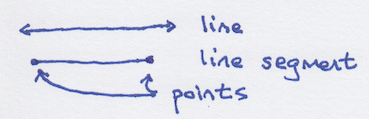
\includegraphics [scale=0.6] {B1.png} \end{center}

Technically, if a line segment is extended (to infinity) in both directions it is called a line and should be represented using arrows on the ends of the part that we draw.  We won't often do that.

Sometimes I may refer to a line segment as a line, as a shorthand, especially when a given statement is true for both lines and line segments.
\begin{center} 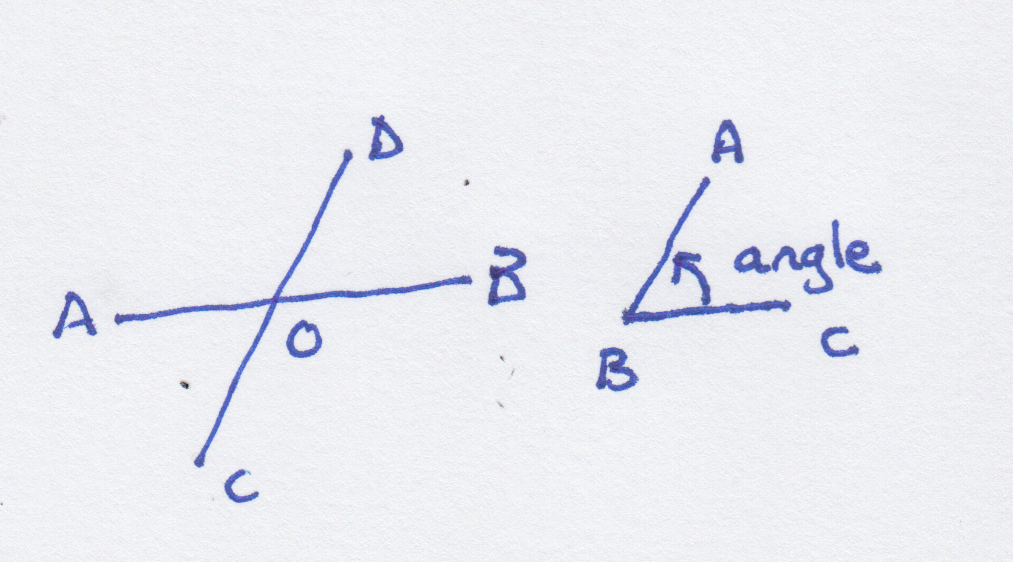
\includegraphics [scale=0.8] {B2b.png} \end{center}
On the left above, four angles are formed when two lines cross at the point $O$.  An angle can also be constructed from line segments.  

On the right, the angle $ABC$, written $\angle ABC$. has its \emph{vertex} at the point $B$.  If there is only one angle for a vertex, I would rather refer to it as $\angle B$ rather than $\angle ABC$.  This is not standard usage, but I think it's easier to comprehend.

Angles have measure, a number which describes how "large" they are.  In the figure above, $\angle AOD$ is larger or "greater" than $\angle DOB$.  

The sum of all the angles around a given point is equal to four right angles.  In a different system of measurement, it is $360{^{\circ}}$ or just 360.  We are not going to use the degrees symbol  ${^{\circ}}$ here.  We say that 360 is equal to four right angles.

The choice of the number 360 is ancient. It's tempting to relate it to the length of the year (approximately 360 days).  Probably it has as much to do with the fact that $2,3,4,5,6,8,9,10,12,15,18,20$ and so on are all factors of $360$, so it can be divided up evenly in many ways.  

You can try to imagine slicing a pizza up into 360 equal slices.  Then the measure of an angle could be determined by how many tiny slices we can fit between the two adjacent sides.  This is basically what a protractor does.

To make it more practical, you could cut slices of size 30, 15 and 5 as well.

\begin{center} 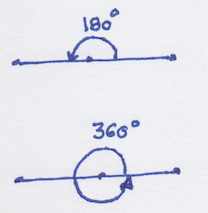
\includegraphics [scale=0.7] {B3.png} \end{center}
The sum of all the angles on one side of a line is half of 360, namely $180$ or two right angles.  Here, we have measured the angles starting from the line segment on the right of the central point.

Angles on one side of a line add up to $180$ (two right angles) even when the angles are not right angles.
\begin{center} 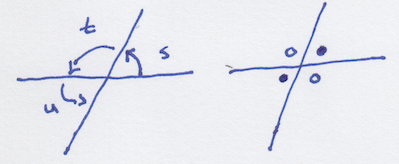
\includegraphics [scale=0.7] {B5.png} \end{center}

In the figure above, $s$ and $t$ are adjacent and lie above the horizontal line --- they add up to $180$.  But $t$ and $u$ are both to the left of the (nearly) vertical line.  So the sum $t + u$ is \emph{also} equal to $180$.
\[ s + t = 180 = t + u \]
subtracting $t$ from both sides:
\[ s = u \]

This leads to a theorem, a true statement that we have deduced, given certain assumptions.  Most of geometry will consist of proving theorems based on a few assumptions, as well as theorems that have already been proved.

$\bullet$  \ $s$ and $u$ are \emph{vertical} angles.  Vertical angles are equal.

In the figure above, there is also a vertical angle corresponding to $t$, which is marked equal on the right by the open circle.

The angles $s$ and $t$ which add to $180$ are called \emph{supplementary} angles.  The theorem we just proved is a consequence of the fact that 

$\bullet$  \ Two angles which are supplementary to the same angle are equal to each other.

\begin{center} 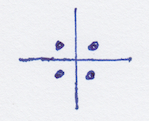
\includegraphics [scale=0.7] {B6b.png} \end{center}
It follows that when two lines cross and one angle is a right angle, all four angles are equal and right angles.

\subsection*{Parallel postulate}

Let's return to parallel lines.  The \emph{parallel} postulate states that if a third line crosses two parallel lines, it forms the same angles with both.  

Our first example is a right angle, and I think you'll agree that this idea makes intuitive sense.  It is like the grid of streets in a standard city layout.
\begin{center} \includegraphics [scale=0.7] {B9b.png} \end{center}

Suppose we had one line crossing two other lines and at the first crossing the angles were all equal, all right angles, but at the second line the angles were not.  If the sum was less than $180$ on one side the two lines would eventually meet on that side.  These would not be parallel lines.

Here is the crucial idea behind the parallel postulate.  Even if the angle formed is not a right angle, it will still be the case that the angles labeled $\theta$ and $\phi$ add up to $180$ or two right angles.
\begin{center} \includegraphics [scale=0.7] {B10b.png} \end{center}

$\bullet$  \ The internal angles on one side of a traversal of two parallel lines always add up to exactly two right angles.

There are altogether two sets of four equal angles in the figure above.  Can you find them?

We combine what we've said up to now.  Red and black add up to $180$.  In the left panel, the two angles marked with black dots are \emph{alternate interior angles}.
\begin{center} 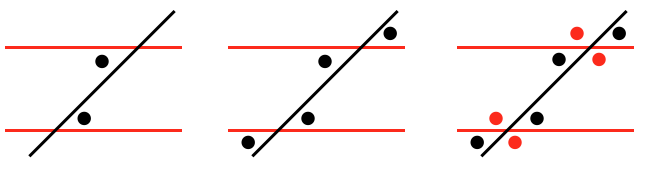
\includegraphics [scale=0.4] {lines_angles_4.png} \end{center}

$\bullet$  \ For a traversal of two parallel lines, alternate interior angles are equal.

The second statement is the converse of the first.  

$\bullet$  \ For a traversal of two lines, if alternate interior angles are equal, the two lines are parallel.

These theorems are important in nearly every proof in elementary geometry:  vertical angles, supplementary angles, and alternate interior angles of parallel lines.

A shorthand way of writing the alternate interior angles theorem is:
\[ \text{alternate interior angles equal} \ \iff \parallel \]
The symbol $\iff$ means \emph{if and only if}.

\subsection*{triangle sum}

$\bullet$ \ The sum of angles in any triangle is 180

You've probably seen this fact at some point, and we'll develop an elegant proof of it later.  Here is a simple arithmetic proof.

Imagine that we walk along the sides of a triangle, turning at each vertex to follow the new side.  It seems pretty clear that the sum of all three turns is 360, which we'll write as twice 180.
\begin{center} 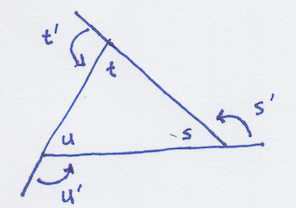
\includegraphics [scale=0.6] {D11.png} \end{center}
\[ s' + t' + u' = 2 \cdot 180 \]

By the supplementary angle theorem, we have three sets of angles, each pair of which adds up to 180, so the three pairs should sum to 3 times 180.
\[ s + s' + t + t' + u + u' = 3 \cdot 180 \]
If we subtract the first from the second:
\[ s + t + u = 180 \]

$\square$

We put a little square at the end to show we're done with the proof.

\subsection*{reflection}

The vertical angles theorem already gives us insight into problems.  As an example, consider the path that light takes going from a source at $A$ to your eye at $B$, reflected in a mirror.  

A pastoral equivalent might be the shepherd who decides to water his flock at the river and then make it back to the barn at $B$ by the shortest path.  Light also takes the shortest path from $A$ to $B$.

\begin{center} \includegraphics [scale=0.5] {Acheson_G46.png} \end{center}

The question is, what is the angle for the shortest path?  

Let us change the problem and tackle it in reverse.  Suppose we place a point $B'$ on the other side of the mirror or across the river.  Not worrying about the barrier, what is the shortest distance from $A$ to $B'$.  It's a straight line, by definition.

But then construct two triangles with the same sides that are mirror images.  We will say more about our methods for proving that the two triangles are identical (allowing mirror images), in the next chapter.

Clearly the distance from $A$ to $B'$ is the same as the distance from $A$ to the mirror and then back to $B$.

At the same time, $\angle \theta$ is equal to the dotted angle below it, and that angle is equal to the angle made by the light coming from $A$, by vertical angles.

We have the \emph{law of reflection}, that for the shortest path, the angle of incidence is equal to the angle of reflection.

\end{document}
